\documentclass[24pt, a4paper, portrait]{article}

\usepackage[utf8]{inputenc}
\usepackage[pages=some]{background}

\usepackage[a4paper,left=2cm,right=2cm,top=1cm,bottom=2cm]{geometry}

\usepackage{graphicx}
\usepackage{array}

\graphicspath{{./img/}}

\begin{document}

\pagestyle{empty}

\raggedleft


\includegraphics[width=0.4\textwidth]{logo}

\vspace{1cm}
\sffamily
\centering
\Huge

\textbf{Hygienehinweise}

%\vspace{1cm}

\raggedright
\huge

\begin{tabular}{ m{3.7cm} m{12.5cm} }
    
\includegraphics[width=3cm]{handhygiene} & Vor und nach der Arbeit im Labor gründlich Hände waschen! \\
    \vspace{2mm}
    
\includegraphics[width=3cm]{desinfektion} & Vor und nach der Arbeit alle benutzten Flächen und Geräte desinfizieren! \\
    \vspace{2mm}
    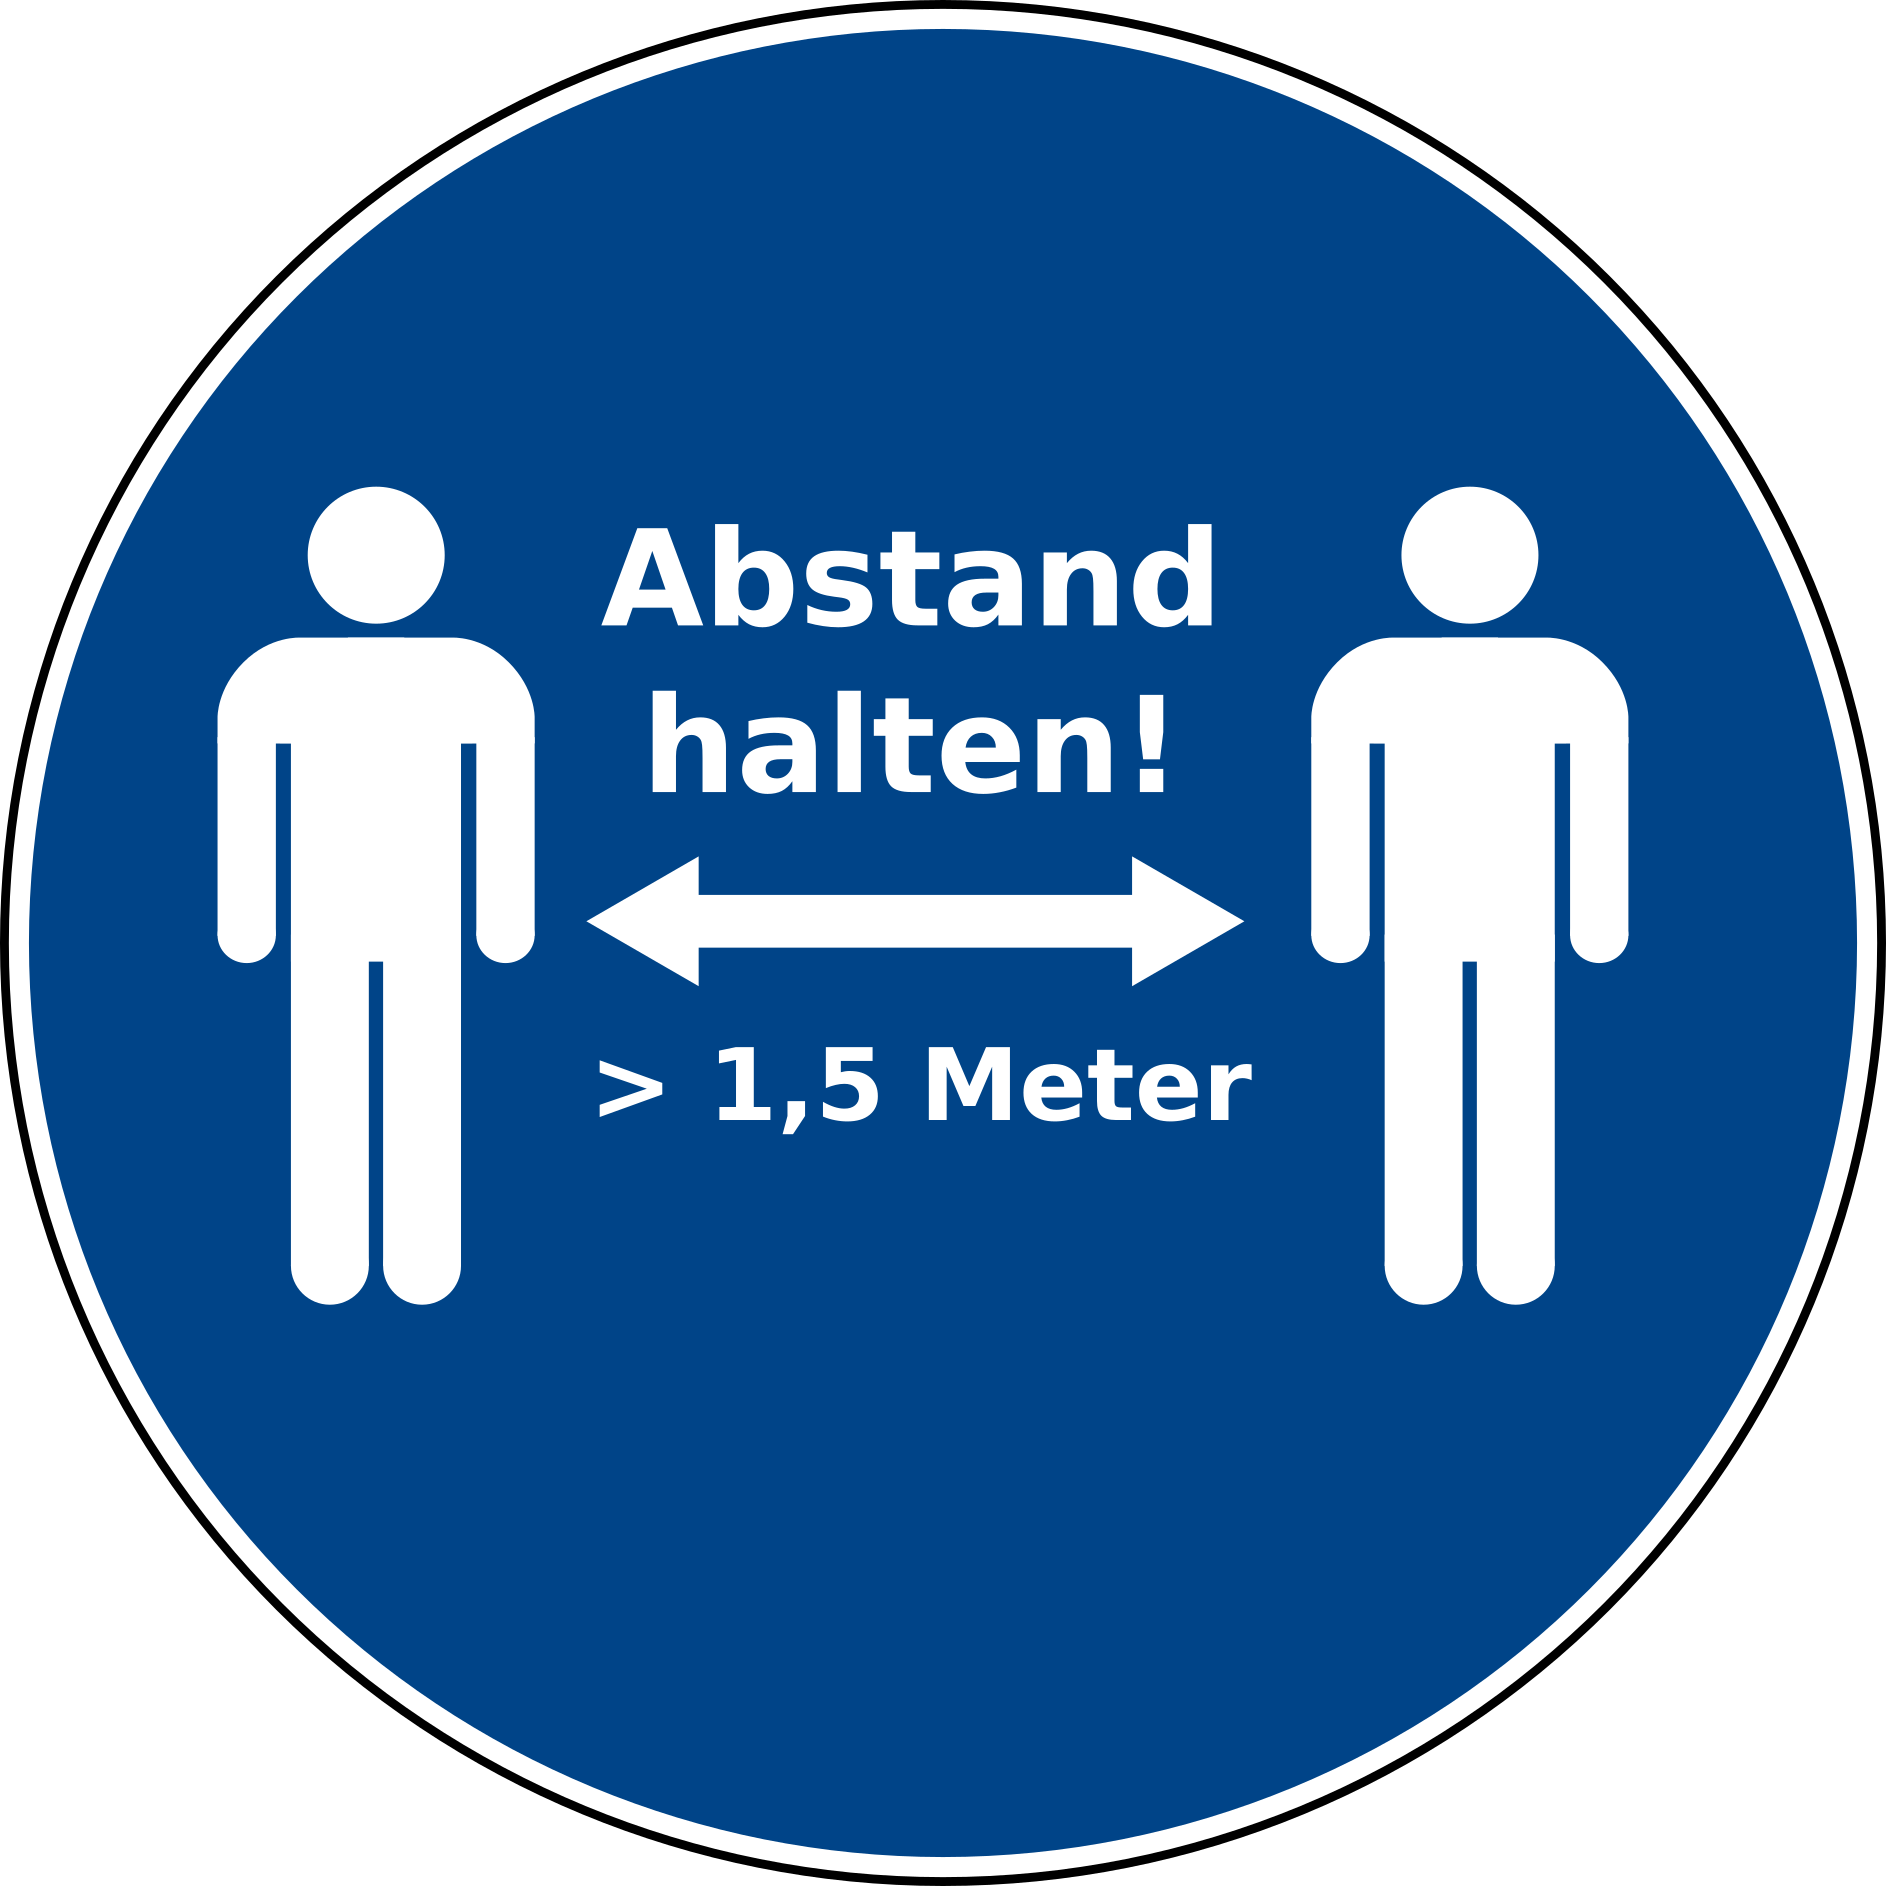
\includegraphics[width=3cm]{abstand} & Stets einen Mindestabstand von 1,5 Metern einhalten! \\
    \vspace{2mm}
    
\includegraphics[width=3cm]{niesetikette} & Beim Niesen und Husten wegdrehen und in die Armbeuge niesen oder husten! \\
    \vspace{2mm}
    
\includegraphics[width=3cm]{maskenpflicht} & FFP2-Maskenpflicht! \\
    \vspace{2mm}
    
\includegraphics[width=3cm]{2g} & Zutritt nur mit vollständigem Impfschutz oder überstandener Corona-Infektion! \\
\end{tabular}


\end{document}
